\chapter{Landmark Graph Construction}\label{Chap:3}
\begin{defn}[\emph{Landmark}]\label{Def:ldmk}
A landmark is a road segment that is frequently traversed by taxi drivers according to the taxi GPS trajectory database. \cite{TDR10}
\end{defn}

The concept of a landmark is proposed primarily for two reasons. First, as mentioned in Section~\ref{Sec:limitation}, the taxi GPS trajectories do not necessarily cover every road segment in a city's road network and the low-sampling-rate problem makes determining the exact route on which a taxi traversed difficult. Therefore, it is not possible to estimate the time cost for each road segment. However, ignoring the length of a road segment and considering it as an abstract ``landmark'' make estimating the travel time between two \emph{landmarks} viable. 

Moreover, the notion of landmarks closely follows the way how drivers remember the driving routes in daily life\cite{TDR10}. For instance, a driving route could be described as ``go straight on the 4th Avenue, turn right at the 7th Street and exit at the Smith Road''. Drivers tend to use familiar road segments as landmarks to guide their directions.

This chapter describes the procedures for constructing a landmark graph in order to estimate the time cost between two landmarks. But before that, the taxi GPS trajectories must be separated into a set of \emph{trips}.

\section{Trip Identification}
\begin{defn}[\emph{Trip}]\label{Def:trip}
A trip is a taxi trajectory that satisfies either condition:
\begin{enumerate}
\item A passenger is on the taxi, namely, all records in the set have an OCCUPIED field of value 1 or, 
\item No passenger is on board, but the time span between \emph{any} two consecutive records is no larger than 3 minutes.
\end{enumerate}
\end{defn}

Table~\ref{Ta:trip_identification} gives a tiny example of trip identification.

\begin{table}[h]
\centering
\resizebox{\columnwidth}{!}{
\begin{tabular}{ | l | l | l | l | l | l | l | l | l | l | l | l | l | }
\hline
\textbf{CUID} & \textbf{UTC} & \textbf{GPS\_LONG} & \textbf{GPS\_LAT} & \textbf{OCCUPIED} & \textbf{TRIP\_ID} \\\hline
1	&	1/5/2009 0:02:00	&	116.39616	&	39.81294	&	0	&	4552265\\ \hline
1	&	1/5/2009 0:04:00	&	116.39575	&	39.82296	&	0	&	4552265\\ \hline
1	&	1/5/2009 0:07:00	&	116.39567	&	39.82774	&	0	&	4552265\\ \hline
1	&	1/5/2009 17:08:00	&	116.30142	&	39.98105	&	1	&	1\\ \hline
1	&	1/5/2009 17:10:00	&	116.29514	&	39.98419	&	1	&	1\\ \hline
1	&	1/5/2009 17:11:00	&	116.28959	&	39.98289	&	1	&	1\\ \hline
1	&	1/5/2009 17:12:00	&	116.28087	&	39.97552	&	1	&	1\\ \hline
1	&	1/5/2009 17:16:00	&	116.26813	&	39.93537	&	1	&	1\\ \hline
1	&	1/5/2009 18:11:00	&	116.36537	&	39.95019	&	0	&	4552271\\ \hline
1	&	1/5/2009 18:12:00	&	116.36546	&	39.94886	&	0	&	4552271\\ \hline
1	&	1/5/2009 18:13:00	&	116.35927	&	39.94528	&	0	&	4552271\\ \hline
\end{tabular}}
\caption{An example of trip identification}\label{Ta:trip_identification}
\end{table}

Clearly, all records in Table~\ref{Ta:trip_identification} belong to one taxi (taxi with CUID = 1) and are sorted chronologically. The first three records, although no passengers are aboard, are considered to be in the same \emph{trip} because the time span between any two consecutive records is no larger than 3 minute. The next five records constitute another trip, even though the last two records have a time difference of 4 minutes, since a passenger is on the taxi (OCCIPIED = 1). Following the same reasoning as the first three's, the last three records are treated as one trip. Listing~\ref{List:code_trip} gives the pseudocode for trip identification.

\begin{lstlisting}[language = Python, caption = {Pseudocode for trip identification}, label = {List:code_trip} ,frame=single, numbers=left,stepnumber=1]
curr_tripid = 1
last_occup = curr_occup = records[0].OCCUPIED
last_unixepoch = curr_unixepoch = records[0].UNIX_EPOCH
for recd in records:
	curr_occup = recd.OCCUPIED
	curr_unixepoch = recd.UNIX_EPOCH
	if curr_occup != last_occup:
		++curr_tripid
	elif (curr_occup == 0) && \
	(curr_unixepoch - last_unixepoch > threshold):
		++curr_tripid
	recd.TRIP_ID = curr_tripid
	last_occup = curr_occup
	last_unixepoch = curr_unixepoch
\end{lstlisting}

It is noteworthy that although the middle five records with OCCUPIED = 1 come chronologically after the first three records, they are nevertheless assigned a smaller TRIP\_ID. This is due to an adjustment made to the actual implementation of the algorithm. The \emph{actual} algorithm operates in two stages. It first identifies trips for all records with OCCUPIED = 1; only in the second stage does it identify trips for records with OCCUPIED = 0. The rationale for this arrangement is to give priority to the records with passengers aboard, because \textbf{these records are guaranteed to belong to one trip}. In fact, the second condition for identifying trips in Definition~\ref{Def:trip} is more of a heuristic rather than a theorem. It is meant to provide sufficient data for subsequent machine learning tasks with reasonable accuracy.

\section{Landmark Frequency}

\begin{table}[h]
\centering
\resizebox{\columnwidth}{!}{
\begin{tabular}{ | l | l | l | l | l | l | l | l | l | l | l | l | l | }
\hline
\textbf{CUID} & \textbf{UTC} & \textbf{GPS\_LONG} & \textbf{GPS\_LAT} & \textbf{Street} & \textbf{TRIP\_ID} \\\hline
1	&	1/5/2009 0:02:00	&	116.39616	&	39.81294	&	A	&	4552265\\ \hline
1	&	1/5/2009 0:04:00	&	116.39575	&	39.82296	&	A	&	4552265\\ \hline
1	&	1/5/2009 0:07:00	&	116.39567	&	39.82774	&	B	&	4552265\\ \hline
1	&	1/5/2009 17:08:00	&	116.30142	&	39.98105	&	C	&	1\\ \hline
1	&	1/5/2009 17:10:00	&	116.29514	&	39.98419	&	C	&	1\\ \hline
1	&	1/5/2009 17:11:00	&	116.28959	&	39.98289	&	C	&	1\\ \hline
1	&	1/5/2009 17:12:00	&	116.28087	&	39.97552	&	A	&	1\\ \hline
1	&	1/5/2009 17:16:00	&	116.26813	&	39.93537	&	A	&	1\\ \hline
1	&	1/5/2009 18:11:00	&	116.36537	&	39.95019	&	B	&	4552271\\ \hline
1	&	1/5/2009 18:12:00	&	116.36546	&	39.94886	&	C	&	4552271\\ \hline
1	&	1/5/2009 18:13:00	&	116.35927	&	39.94528	&	C	&	4552271\\ \hline
\end{tabular}}
\caption{An illustration of frequency counting}\label{Ta:frequency_count}
\end{table}

Definition~\ref{Def:trip} states that whether recognising a particular road segment as a landmark or not is based on some notion of frequency. Only if a road segment is visited by drivers frequently enough is it recognised as a landmark. In this project, the notion of frequency is given by Definition~\ref{Def:frequency}.

\begin{defn}[\emph{Frequency of a Road Segment}]\label{Def:frequency}
The frequency of a road segment is the sum of \emph{unique} occurrences of that road segment in each trip. 
\end{defn}

Table~\ref{Ta:frequency_count} illustrates how the frequency of a road segment is calculated. In Trip 4552265, Street A occurs twice but \textbf{its frequency increases only by one}. Similarly, Street C occur three times and Street A occur twice in Trip 1, but \textbf{their occurrences only add one to their frequencies}. Therefore, even though Street B \emph{appears} less times than Street A or Street C, \textbf{all streets have the same frequency of 2}, based on this set of records.  

The algorithm for counting frequency of a road segment is rather straightforward as in Listing~\ref{List:code_frequency}.

\begin{lstlisting}[language = Python, caption = {Pseudocode for counting road frequency}, label = {List:code_frequency} ,frame=single, numbers=left, stepnumber=1]
frequencies = dict{}
for trip in trips:
 	// get unique streets
	streets = unique(trip.streets)
	for street in streets:
		if street in frequencies:
			++frequencies[street]
		else:
			frequencies[street] = 1
\end{lstlisting}

After the frequency of each road segment is determined, a parameter $k$ is set to select the top $k$ frequent road segments as \emph{landmarks}. For this project, $k$ was chosen to be 500 to ensure the road segments are significant enough to be landmarks. When plotted on a map, these 500 landmarks cover most of the main streets in Beijing as shown in Figure~\ref{Fig:ldmk_500}. 

\begin{figure}[h]
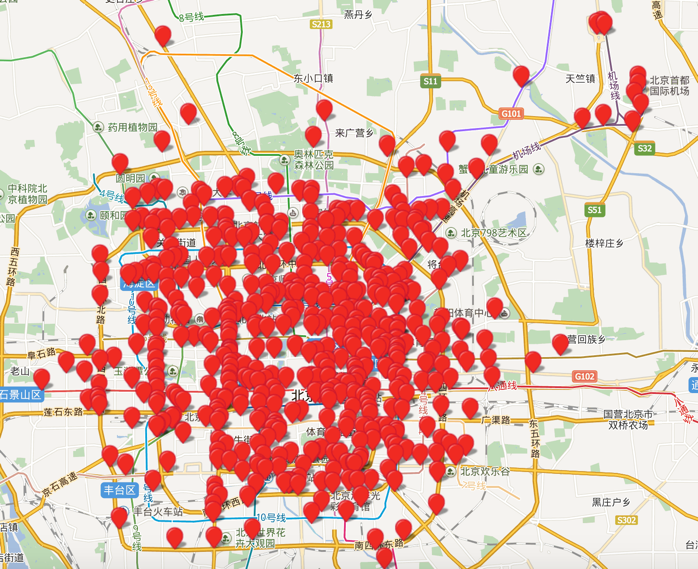
\includegraphics{ldmk_plot}
\centering
\caption{A plot of landmarks when $k$ = 500}\label{Fig:ldmk_500}
\end{figure}

\section{Landmark Graph}\label{ldmk_graph}
\begin{defn}[\emph{Landmark Graph}]\label{Def:ldmk_graph}
A landmark graph is a weighted, directed graph $G=(V,E)$ where V is the set of landmarks defined by parameter $k$ and E is the set of taxi trajectories $T = (p_1,p_2,\textellipsis,p_n)$ that satisfy the following conditions:
\begin{enumerate}
\item $p_1$ and $p_n$ must be landmarks; 
\item $p_2, p_3, \textellipsis , p_{n-1}$ must \textbf{not} be landmarks and;
\item The duration of the trajectory must \textbf{not} exceed a threshold $t_{max}$.
\end{enumerate}
\end{defn}

The threshold $t_{max}$ is used to eliminate trajectories with unreasonably long du\-rations\cite{TDR10}. Sometimes, a taxi may traverse several landmarks but only the first and the last landmarks are recorded, due to the low sampling rate, which cause the duration between the two recorded landmarks to be unreasonably long. For this project, $t_{max}$ was set to 20 minutes. The algorithm for constructing landmark graph is given in Listing~\ref{List:code_ldmk_graph}.

\begin{lstlisting}[language = Python, caption = {Pseudocode for constructing landmark graph}, label = {List:code_ldmk_graph}, frame=single, numbers=left, stepnumber=1]
for trip in trips:
   //get unique, chronologically ordered streets
   streets = unique_ordered(trip.streets)
   while j < len(streets):
	//loop until a landmark is found
	while j < len(streets) && !is_landmark(streets[j]):
		j = j + 1
		
	intermediaries = []
	//find another landmark
	k = j + 1
	while k < len(streets) && !is_landmark(streets[k]):
		intermediaries.append(streets[k])
		k = k + 1
		
	//insert edge (streets[j], intermediaries, streets[k])
	insert(E, streets[j], intermediaries, streets[k])
		
	//next search starts from the second landmark
	j = k
\end{lstlisting}
